% Chapter Template

\chapter{Agile and Correct by Construction} % Main chapter title

\label{Chapter 2} % Change X to a consecutive number; for referencing this chapter elsewhere, use \ref{ChapterX}

%----------------------------------------------------------------------------------------
\section{Correct by Construction development workflow}

The main properties of the CbyC development process are  \parencite{Tokeneer}:
\begin{itemize}
	\item each life-cycle phase can be validated;
	\item the semantic gap between life-cycle phases are reduced, making it possible
		to show the conformance of later life-cycle phases with earlier phases.
\end{itemize}

The CbyC development process products are shown in Figure \ref{fig:CbyCDev}. We now describe each product and how it is created.

\begin{figure}[H]
	\centering
	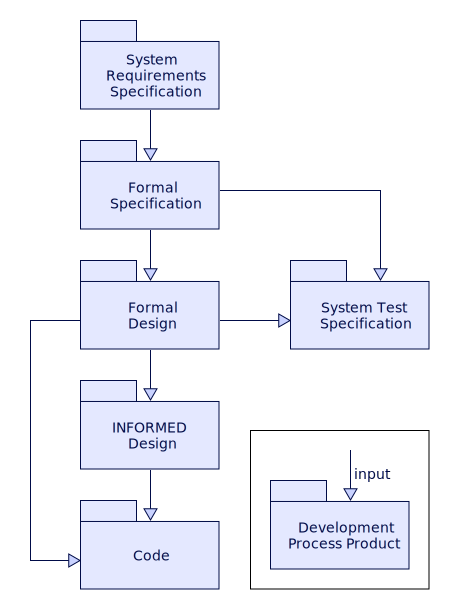
\includegraphics[scale=0.75]{Figures/CbyC_process.pdf}
	\decoRule
	\caption{CbyC development process products.}
	\label{fig:CbyCDev}
\end{figure}

\subsection{System Requirements Specification}

The ``System Requirements Specification'' development process product is the result
of the requirements analysis process.

The aim of requirements analysis is to identify the needs of the stakeholders, 
the desired behaviour of the system, and any non-behavioural characteristics that are needed \parencite{Tokeneer}. 

Requirements management extends throughout the system's development, but it is 
most significant at the beginning, where it is used to identify \parencite{Tokeneer}:
\begin{itemize}
	\item the stakeholders, who have an interest in the development and use of the system
	\item the system boundary, to clarify the scope of the project and the interfaces to external systems
	\item the expected use, in terms of interactions between users and the system
	\item system properties, such as security properties, performance properties, etc.
\end{itemize}

Every requirement should be traceable through each level of system representation (requirements, specification, design, code, test) \parencite{Tokeneer}.

The reasons for producing the System Requirements Specification are \parencite{Tokeneer}:
\begin{itemize}
	\item To early in the project clarify the system's boundary (what is in scope 
		and what is out of scope, and the interfaces necessary to external systems).
	\item To agree on the system requirements with all of the stakeholders.
	\item To document the requirements in a sufficiently precise manner to allow 
		subsequent development of the formal specification to proceed smoothly with 
		little customer input.
	\item To clarify and document the assumptions about the behaviour of external 
		systems, a common source of error.
	\item To identify and manage conflicting expectations between stakeholders.
\end{itemize}

\subsection{Formal Specification}

The aim of the Formal Specification is to unambiguously describe what the system
will do. It should enable the developer and the client to gain a common
understanding of what the system will do \parencite{Tokeneer}.

The abstraction level is important. The formal specification should not address 
how the system is implemented, internal details are deliberately left very abstract. 
Interactions with the external environment are specified, but may be left abstract \parencite{Tokeneer}.

The Formal Specification is written in mathematical notation with an English 
narrative. The specification is divided into small components that can be reasoned
about individually and then combined to describe the system as a whole \parencite{Tokeneer}.

The reasons for producing a Formal Specification are \parencite{Tokeneer}:
\begin{itemize}
	\item It provides an unambiguous description of what the system does. This is
		important for gaining client approval of the behaviour of the system to be
		developed.
	\item It is demonstrably complete.
	\item It can be formal verified, i.e. it can be proved consistent.
\end{itemize}

\subsection{Formal Design}

The aim of the formal design is to elaborate the abstract aspects of the Formal 
Specification to explain how the system will be implemented. The Formal Design 
describes the system in terms of concrete state and operations using types that
are easily implemented. The Formal Design is the source of the required functional
behaviour used during implementation  \parencite{Tokeneer}.

The design is written in the same mathematical notation as the Formal Specification.
This means that the design can be formally verified and errors can be uncovered
before implementation starts \parencite{Tokeneer}.

The reasons for producing a Formal Design are  \parencite{Tokeneer}:
\begin{itemize}
	\item It provides an unambiguous description of how the system does what the formal specification requires.
	\item It can be shown to be complete.
	\item It can be formal verified, i.e. it can be proved consistent.
\end{itemize}

\subsection{System Test Specification}

The aim of the System Test it to demonstrate that the system has the correct 
behaviour as specified in the Formal Specification. This differs from the goals of
acceptance testing which is designed to demonstrate that the System meets
its requirements. System Testing aims to achieve 100\% coverage of the formal 
specification. Thus so all possible behaviours described in the formal specification
should be exercised at least once \parencite{Tokeneer}.

The Formal Design is a refinement of the Formal Specification. Therefore the Test
Specification can also be written against the Formal Design if you want to tests 
details of the design \parencite{Tokeneer}.

All System tests are specified in a System Test Specification prior to their 
execution.  The tests are specified as scenarios that might occur in typical usage
of the system. The specification includes documentation of the expected outcome
of the test. System test specifications also traces each test to the components
of the Formal Specification/Design that the test attempts to exercise \parencite{Tokeneer}.

Where code coverage metrics need to be captured, this is be done during the
System test. This allows us to question the use of any code that cannot be covered
by a system test. If the code is valid then focused unit tests should be added to
cover the code \parencite{Tokeneer}.

The reasons for producing a System Test Specification are \parencite{Tokeneer}:
\begin{itemize}
	\item A system test focuses on testing the behaviour of the whole system against
		the expected (specified) behaviour.
	\item A system test is likely to find faults caused by the incorrect interaction
		of modules within the system.
	\item System testing complements static analysis, in that it confirms the 
		dynamic behaviour.
\end{itemize}

\subsection{INFORMED Design}
CbyC design methodology is based on information flow. The information flow is 
defined using a contract-based notation. The contract-based notation is used to
define the abstract state of the program and the information relationships across
boundaries \parencite{CbyCMan}.

Consideration of information flows at the design stage leads to programs with the
desirable properties of abstraction, encapsulation, high cohesion and loose 
coupling \parencite{Tokeneer}.

The \textbf{IN}formation \textbf{F}low \textbf{OR}iented \textbf{ME}thod of
object \textbf{D}esign (INFORMED) design provided an architectural framework
in which to perform the implementation. Consideration of information flows at the
design stage results in programs with the desirable properties of abstraction, 
encapsulation, high cohesion and loose coupling \parencite{Tokeneer}.

The INFORMED design aids maintenance and upgrades of the software by providing a
route-map from the Formal Design to the code \parencite{Tokeneer}.

The reasons for producing an INFORMED Design are \parencite{Tokeneer}:
\begin{itemize}
	\item It focuses on the system architecture and ensures that the architecture 
		fits the information flow model.
	\item It provides the mapping from the Formal Design to the Code before writing
		the code.
	\item It complements the Formal Design without duplicating functional information.
\end{itemize}

\subsection{Code Implementation}


\section{Manifesto for Agile Software Development}

The manifesto sets out the overarching principles of agile software development \parencite{Beck2001ManifestoFA}:

\begin{displayquote}
We are uncovering better ways of developing software by doing it and helping 
others do it. Through this work we have come to value:

\begin{itemize}
	\item \textbf{Individuals and interactions} \textit{over} processes and tools 
	\item \textbf{Working software} \textit{over} comprehensive documentation 
	\item \textbf{Customer collaboration} \textit{over} contract negotiation 
	\item \textbf{Responding to change} \textit{over} following a plan 
\end{itemize}

That is, while there is value in the items on the right, we value the items on
the left more.
\end{displayquote}


